\section{Toolbox}
% Light emission, ligth absorption, population inversion, stimulated emission

\begin{frame}{Electromagnetic Spectrum}

    \begin{columns}[c, onlytextwidth]

        \begin{column}{0.55\textwidth}

            The energy of a photon is given by the \textbf{Planck's relation}\footnotemark[1]:

            \begin{equation}
                e = h f \quad \text{[eV or J]}
            \end{equation}

        \end{column}

        \begin{column}{0.45\textwidth}

            \begin{figure}
                \centering
                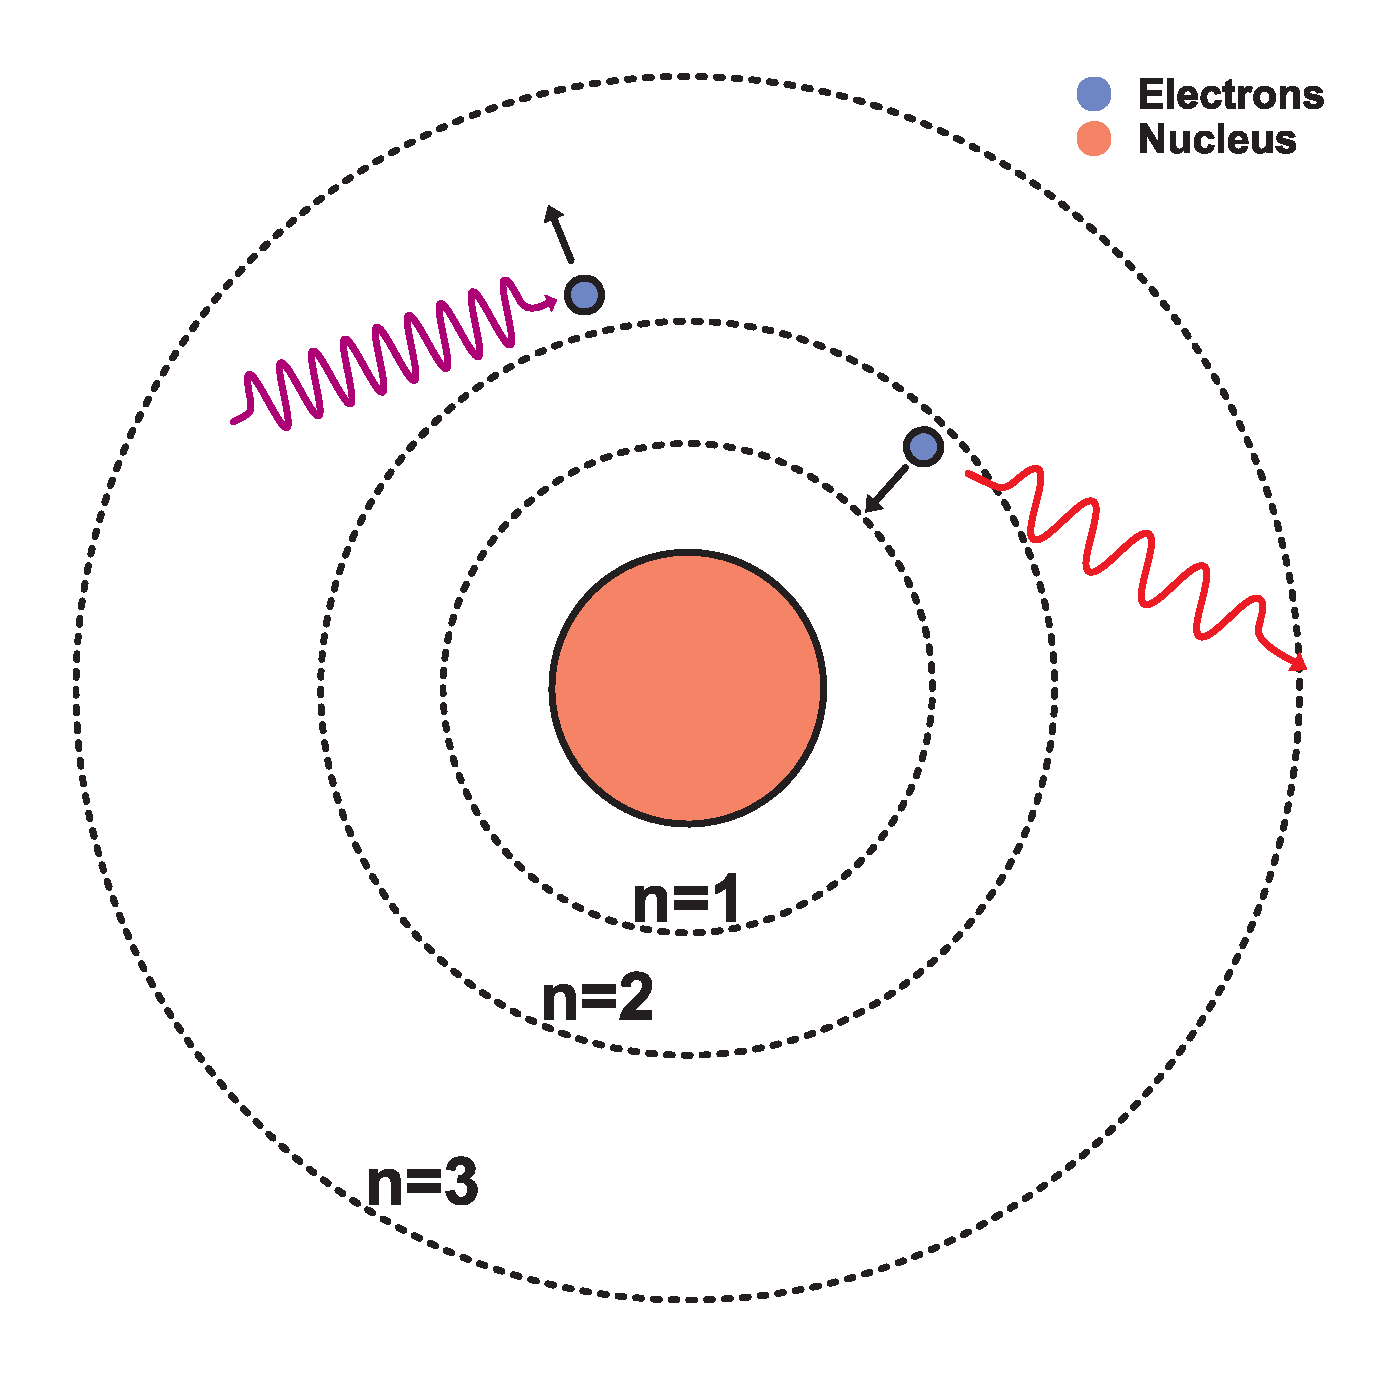
\includegraphics[width=0.9\textwidth]{pdf/eletronic-structure.pdf}
            \end{figure}

        \end{column}

    \end{columns}

    \begin{figure}[H]
        \centering

        \resizebox{\columnwidth}{!}{%
            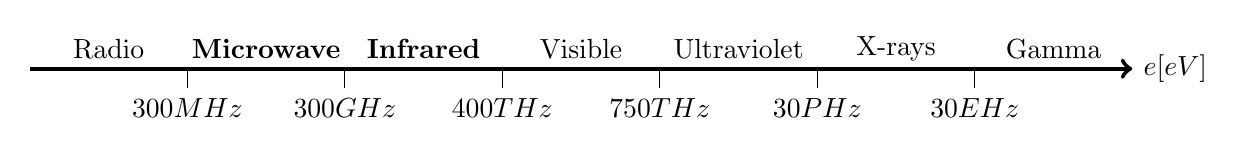
\begin{tikzpicture}[scale=0.5]
                % Spectrum lines
                \draw[ultra thick, ->] (0,0) -> (28,0) node[right] {$e \text{ [eV]}$};

                % Wavelengths
                \foreach \w/\label in {4/$300MHz$, 8/$300GHz$, 12/$400THz$, 16/$750THz$, 20/$30PHz$, 24/$30EHz$}
                    {
                        \draw (\w,0) -- (\w,-0.5) node[below] {\label};
                    }

                % Labels
                \foreach \w/\label in {2/Radio, 6/\textbf{Microwave}, 10/\textbf{Infrared}, 14/Visible, 18/Ultraviolet, 22/X-rays, 26/Gamma}
                    {
                        \node at (\w, 0.5) {\label};
                    }

            \end{tikzpicture}
        }

    \end{figure}

    Our working frame will be in the \textbf{microwave} and \textbf{infrared} regions.

    \footnotetext[1]{Planck's constant $h = 6.62607015 \times 10^{-34} \text{J s}$}

\end{frame}



\begin{frame}{Rubidium and Cesium}

    We will deal with Rubidium (isotopes $^{85}Rb$ \& $^{87}Rb$) and Cesium ($^{133}Cs$).

    \begin{itemize}
        \item They are both alkali metals with a single valence electron.
        \item Their first ionization energy is low.
    \end{itemize}

    \begin{columns}[c, onlytextwidth]

        \begin{column}{0.5\textwidth}

            \begin{figure}
                \centering
                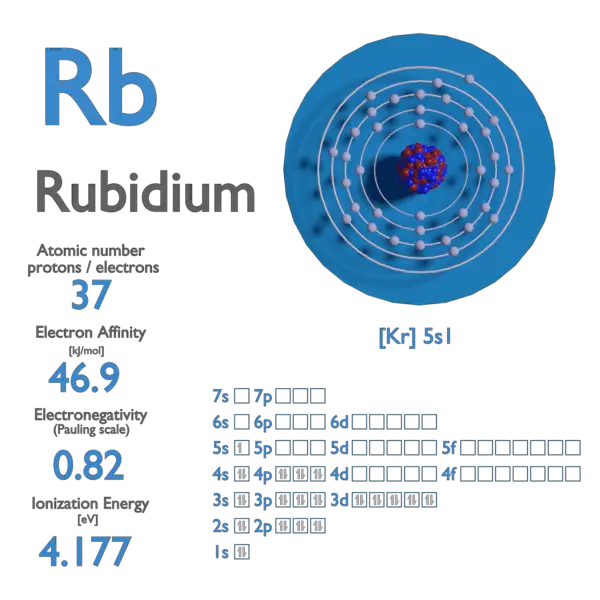
\includegraphics[width=0.8\textwidth]{img/data-Rubidium.png}
            \end{figure}

        \end{column}

        \begin{column}{0.5\textwidth}

            \begin{figure}
                \centering
                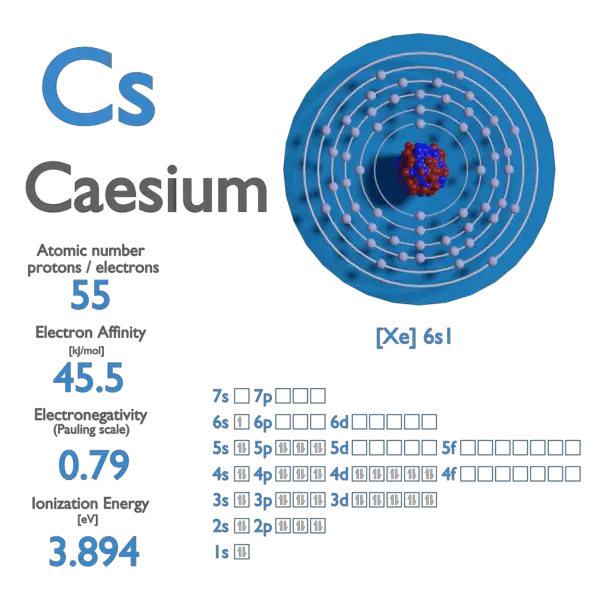
\includegraphics[width=0.8\textwidth]{img/data-Caesium.png}
            \end{figure}

        \end{column}

    \end{columns}

\end{frame}



\begin{frame}{Quantum levels}

    \begin{columns}[c, onlytextwidth]

        \begin{column}{0.45\textwidth}

            \begin{figure}
                \centering
                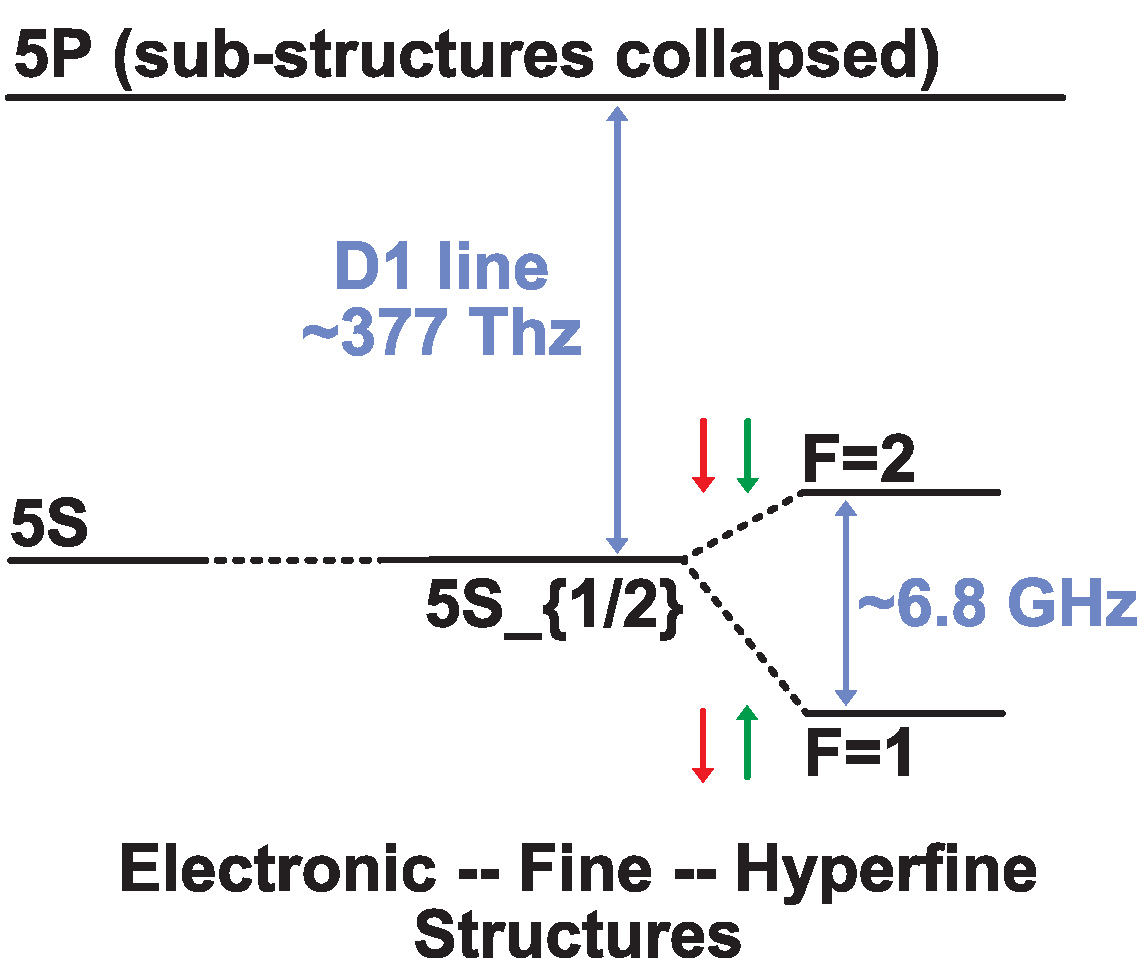
\includegraphics[width=0.8\textwidth]{pdf/Rubidium-hyperfine-levels.pdf}
                \caption{$^{87}Rb$ quantum levels.}
            \end{figure}

        \end{column}

        \begin{column}{0.55\textwidth}

            \textbf{Elementary energy level ($n=1,2,3,\ldots$), can further be split.\footnotemark[1]}

            \vspace{10pt}

            Substructures are due to various quantum phenomena acting inside the atom domain.

            \begin{itemize}
                \item Electronic str.: classical orbital levels.
                \item Fine str.: electronic spin-orbit coupling.
                \item Hyperfine str.: \textcolor[HTML]{FF0000}{nuclear spin}-\textcolor[HTML]{00ED00}{electron spin} coupling.
            \end{itemize}

        \end{column}

    \end{columns}

    \vspace{10pt}

    \footnotetext[1]{For the purpose of the CSACs, we can consider the sub-$5P$ structures as collapsed into a single one.}

\end{frame}



% \begin{frame}{Optical pumping}
% \end{frame}